\subsection{Sférická dutina obalená $\delta$-slupkou}
	Částice se rozptyluje na potenciálu
	\begin{equation}
		V(r)
			=\frac{v}{a}\delta(r-a)
	\end{equation}
	(dutina obalená nekonečně tenkou slupkou z $\delta$-funkce).
	
	\begin{itemize}
		\item 
			Nalezněte radiální část vlnové funkce $R_{kl}(r)$.
			
		\item
			Určete fázové posunutí $l$-té parciální vlny $\delta_{l}(k)$.
			
		\item
			Určete totální účinný průřez $l$-té parciální vlny $\sigma_{l}(k)$.
	\end{itemize}

	\begin{solution}
		Až na oblast $\delta$-slupky se jedná o pohyb volné částice.
		Radiální část její vlnové funkce bude mít obecný tvar daný lineární kombinací sférické Besselovy a Neumannovy funkce~\eqref{eq:FreeParticleRadialWF}.
		Uvnitř koule pak musí být
		\begin{equation}
			R_{kl}(r<a)
				=A_{l}(k)j_{l}(kr)
		\end{equation}
		(odůvodnění stejné jako v případě volné částice, 
		vlnová funkce nesmí divergovat v počátku).
		
		Řešení vně koule se zapíše jako
		\begin{equation}
			R_{kl}(r)
				=B_{l}(k)\left[\alpha_{l}(k)j_{l}(kr)+\beta_{l}(k)n_{l}(kr)\right]
		\end{equation}
		což v asymptotice $r\rightarrow\infty$ \eqref{eq:SphericalBesselInfinity} dává
		\begin{equation}
			R_{kl}(r\rightarrow\infty)
				\rightarrow B_{l}(k)\left[\alpha_{l}(k)\,\frac{\sin\left(kr-l\frac{\pi}{2}\right)}{kr}
					-\beta_{l}(k)\,\frac{\cos\left(kr-l\frac{\pi}{2}\right)}{kr}\right]
		\end{equation}
		Asymptotika zcela volné částice, jejíž řešení je \eqref{eq:FreeParticleRadialWF}, zní
		\begin{equation}\label{eq:DeltaShellPotentialRInfinity}
			R_{kl}^{(0)}(r\rightarrow\infty)
				\rightarrow\frac{\sin\left(kr-l\frac{\pi}{2}\right)}{kr}.
		\end{equation}
		Potenciál $\delta$-slupky tedy způsobí fázové posunutí oproti případu volné částice.
        To je dáno veličinou $\delta_{l}(k)$:
		\begin{align}
			R_{kl}(r\rightarrow\infty)
				&\rightarrow\frac{\sin\left(kr-l\frac{\pi}{2}+\delta_{l}(k)\right)}{kr}=\nonumber\\
				&=\cos{\delta_{l}(k)}\,\frac{\sin\left(kr-l\frac{\pi}{2}\right)}{kr}
					+\sin{\delta_{l}(k)}\,\frac{\cos\left(kr-l\frac{\pi}{2}\right)}{kr}
		\end{align}
		Srovnáním s předchozím vyjádřením \eqref{eq:DeltaShellPotentialRInfinity} vychází pro fázové posunutí
        \begin{subequations}
            \begin{align}
                \alpha_{l}(k)
                    &=\cos{\delta_{l}(k)}\\
                \beta_{l}(k)
                    &=-\sin{\delta_{l}(k)}
            \end{align}                
        \end{subequations}
		a vlnovou funkci lze zapsat ve tvaru
		\begin{equation}
			\important{
				R_{kl}(r)=
					\begin{cases}
						A_{l}(k)j_{l}(kr) & \text{pro }r<a\\
						B_{l}(k)\left[\cos{\delta_{l}(k)}j_{l}(kr)-\sin{\delta_{l}(k)}n_{l}(kr)\right] &\text{pro }r>a
					\end{cases}
            }.
		\end{equation}
		
		Fázové posunutí se dopočítá pomocí sešívacích podmínek na $\delta$-slupce.
		Stejně jako v případě jednorozměrného potenciálu i zde musí platit dvě podmínky:
		\begin{enumerate}
			\item
				Vlnová funkce je spojitá,
				\begin{equation}\label{eq:DeltaShellPotentialRContinuity}
					A_{l}(k)j_{l}(ka)
						=B_{l}(k)\left[\cos{\delta_{l}(k)}j_{l}(ka)-\sin{\delta_{l}(k)}n_{l}(ka)\right].
				\end{equation}
					
			\item
				V derivaci je skok daný silou $\delta$-funkce~\eqref{eq:SewDerivativeDelta}
				\begin{equation}
					R'_{kl}(a+0)-R'_{kl}(a-0)
						=\frac{2Mv}{\hbar^{2}a}R_{kl}(a),
				\end{equation}
				což v našem případě dává (pozor, $R'_{kl}=\frac{\d}{\d r}R_{kl}$, tj. derivuje se jen podle $r$)
				\begin{equation}\label{eq:DeltaShellPotentialRJump}
					kB_{l}(k)\left[\cos{\delta_{l}(k)}j'_{l}(ka)-\sin{\delta_{l}(k)}n'_{l}(ka)\right]
						-kA_{l}(k)j'_{l}(ka)
						=\frac{Q}{a}A_{l}(k)j_{l}(ka),
				\end{equation}
				kde se pro zjednodušení zápisu zavedlo $Q\equiv2mv/\hbar^{2}$.
		\end{enumerate}
		
		Dosazení z \eqref{eq:DeltaShellPotentialRContinuity} do \eqref{eq:DeltaShellPotentialRJump} vede na (argumenty funkcí již nejsou explicitně vypsány)
		\begin{align}
			j_{l}j'_{l}\cos{\delta_{l}}-j_{l}n'_{l}\sin{\delta_{l}}
				-j_{l}j'_{l}\cos{\delta_{l}}+j'_{l}n_{l}\sin{\delta_{l}}
				&=\frac{Q}{ka}j_{l}\left(j_{l}\cos{\delta_{l}}-n_{l}\sin{\delta_{l}}\right)\nonumber\\
			-\left(j_{l}n'_{l}-j'_{l}n_{l}\right)\sin{\delta_{l}}
				&=\frac{Q}{ka}j_{l}\left(j_{l}\cos{\delta_{l}}-n_{l}\sin{\delta_{l}}\right).
		\end{align}
		Na levé straně se objevil Wronskián \eqref{eq:SphericalBesselWronskian}, za který se dosadí výsledek předchozího příkladu:
		\begin{equation}
			-\frac{1}{(ka)^{2}}\sin{\delta_{l}}
				=\frac{Q}{ka}j_{l}\left(j_{l}\cos{\delta_{l}}-n_{l}\sin{\delta_{l}}\right)
		\end{equation}
		Explicitní výraz pro fázové posunutí tedy zní
		\begin{equation}\label{eq:DeltaShellPotentialPhaseShift}
			\important{
				\tg\delta_{l}(k)
					=\frac{Qj_{l}^{2}(ka)}{Qj_{l}(ka)n_{l}(ka)-\frac{1}{ka}}
            }.
		\end{equation}

		Z podmínky spojitosti~\eqref{eq:DeltaShellPotentialRContinuity} se dá určit \emph{koeficient průniku}
		\begin{equation}\label{eq:DeltaShellPotentialP}
			P_{l}(k)
				\equiv\abss{\frac{A_{l}(k)}{B_{l}(k)}}
				=\frac{\cos{\delta_{l}(k)}j_{l}(ka)-\sin{\delta_{l}(k)}n_{l}(ka)}{j_{l}(ka)},
		\end{equation}
		kam je potřeba dosadit v tuto chvíli již známé fázové posunutí $\delta_{l}(k)$.

		Jako poslední se určí účinný průřez pro $l$-tou parciální vlnu.
		K tomu se použije vztah \eqref{eq:ScatteringSigmal}.
		Mezi goniometrickými funkcemi platí identita
		\begin{equation}
			\sin^{2}x=\frac{\tg^{2}x}{1+\tg^{2}x},
		\end{equation}
		což v tomto případě dává
		\begin{align}
			\sin^{2}\delta_{l}(k)
				&=\frac{\tg^{2}\delta_{l}(k)}{1+\tg^{2}\delta_{l}(k)}=\nonumber\\
				&=\frac{Q^{2}j_{l}^{4}(ka)}{Q^{2}j_{l}^{4}(ka)+\left[Qj_l(ka)n_{l}(ka)-\frac{1}{ka}\right]^{2}}
		\end{align}
		a účinný průřez je tedy
		\begin{equation}\label{eq:DeltaShellPotentialCrossSection}
			\important{
				\sigma_{l}(k)
					=\frac{4\pi}{k^{2}}(2l+1)
						\frac{Q^{2}j_{l}^{4}(ka)}{Q^{2}j_{l}^{4}(ka)+\left[Qj_l(ka)n_{l}(ka)-\frac{1}{ka}\right]^{2}}
			}
		\end{equation}

		\begin{figure}[!hbp]
            \begin{subfigure}{0.32\linewidth}\centering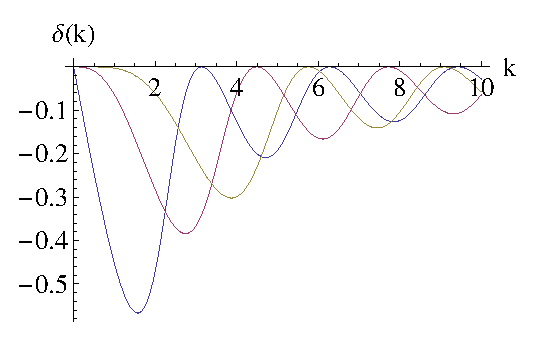
\epsfig{file=figures/delta1.eps,width=\linewidth,keepaspectratio}\end{subfigure}\hfill
            \begin{subfigure}{0.32\linewidth}\centering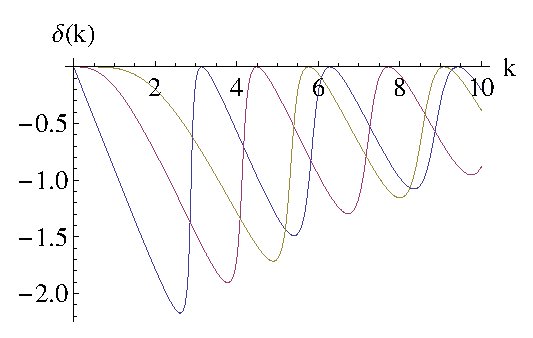
\epsfig{file=figures/delta10.eps,width=\linewidth,keepaspectratio}\end{subfigure}
            \begin{subfigure}{0.32\linewidth}\centering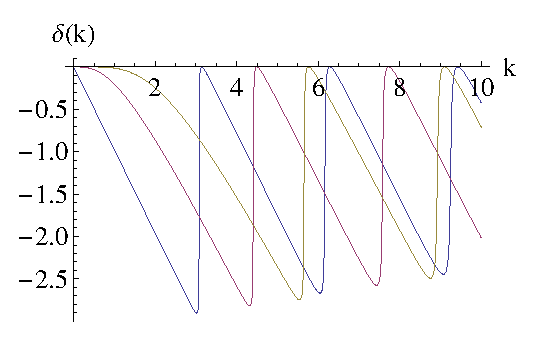
\epsfig{file=figures/delta50.eps,width=\linewidth,keepaspectratio}\end{subfigure}
            \begin{subfigure}{0.32\linewidth}\centering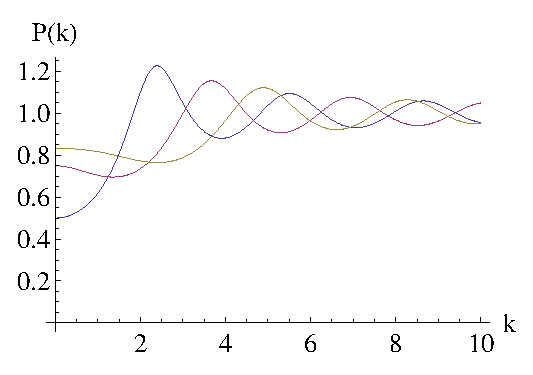
\epsfig{file=figures/P1.eps,width=\linewidth,keepaspectratio}\end{subfigure}\hfill
            \begin{subfigure}{0.32\linewidth}\centering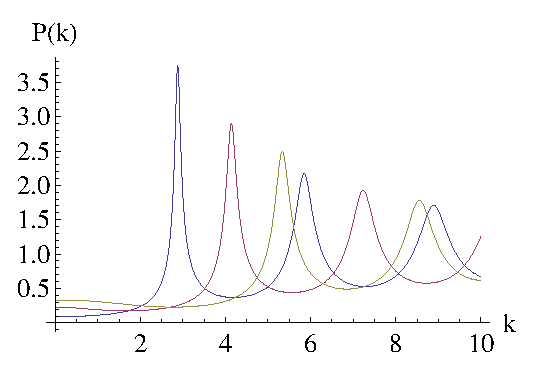
\epsfig{file=figures/P10.eps,width=\linewidth,keepaspectratio}\end{subfigure}
            \begin{subfigure}{0.32\linewidth}\centering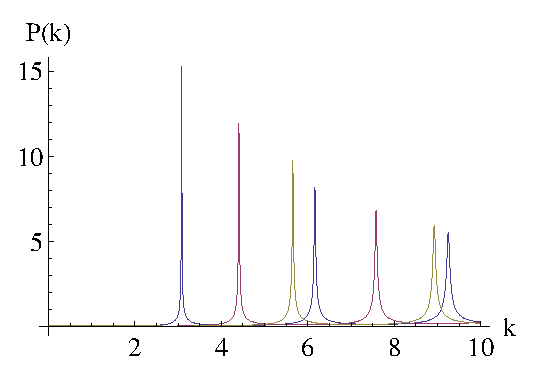
\epsfig{file=figures/P50.eps,width=\linewidth,keepaspectratio}\end{subfigure}
            \begin{subfigure}{0.32\linewidth}\centering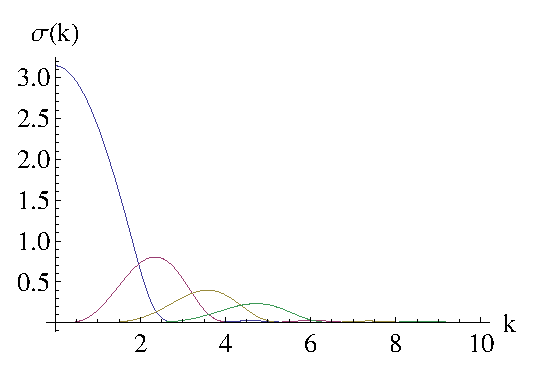
\epsfig{file=figures/sigma1.eps,width=\linewidth,keepaspectratio}\end{subfigure}\hfill
            \begin{subfigure}{0.32\linewidth}\centering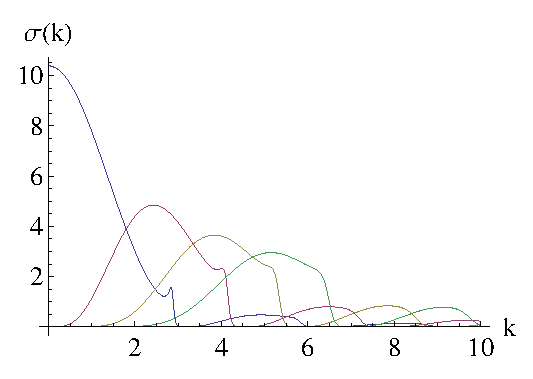
\epsfig{file=figures/sigma10.eps,width=\linewidth,keepaspectratio}\end{subfigure}
            \begin{subfigure}{0.32\linewidth}\centering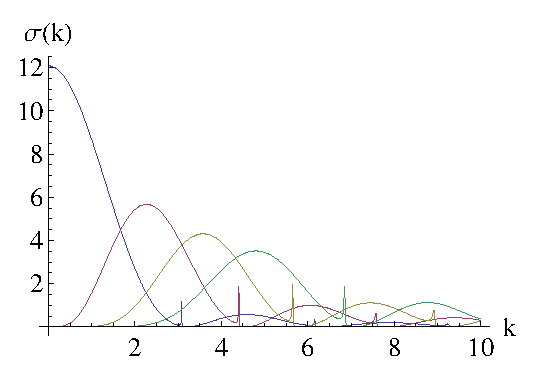
\epsfig{file=figures/sigma50.eps,width=\linewidth,keepaspectratio}\end{subfigure}
            \begin{subfigure}{0.32\linewidth}\centering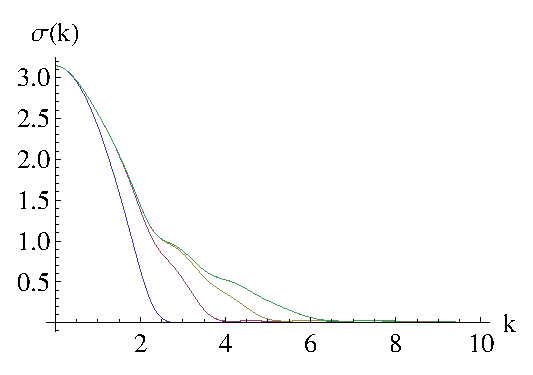
\epsfig{file=figures/sumsigma1.eps,width=\linewidth,keepaspectratio}\end{subfigure}\hfill
            \begin{subfigure}{0.32\linewidth}\centering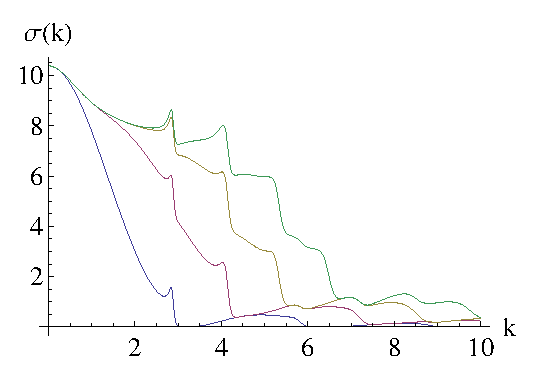
\epsfig{file=figures/sumsigma10.eps,width=\linewidth,keepaspectratio}\end{subfigure}
            \begin{subfigure}{0.32\linewidth}\centering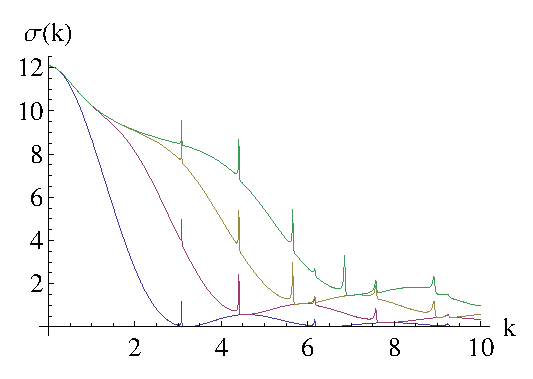
\epsfig{file=figures/sumsigma50.eps,width=\linewidth,keepaspectratio}\end{subfigure}
			
			\scaptionx{Výsledky pro rozptyl na sférické $\delta$-slupce}{	
				{\bf 1. řádek:} 
					Fázové posunutí $l$-té parciální vlny $\delta_{l}(k)$ 
					podle \eqref{eq:DeltaShellPotentialPhaseShift}
					pro $l=0$ (modře), $l=1$ (fialově), $l=2$ (béžově).				
				{\bf 2. řádek:}
					Koeficient průniku $l$-té parciální vlny $P_{l}(k)$ 
					podle \eqref{eq:DeltaShellPotentialP}.
				{\bf 3. řádek:}				
					Účinný průřez $l$-té parciální vlny podle \eqref{eq:DeltaShellPotentialCrossSection}.
				{\bf 4. řádek:}
					Součet účinných průřezů $\sigma_{0}$ (modře), $\sigma_{0}+\sigma_{1}$ (fialově),
					$\sigma_{0}+\sigma_{1}+\sigma_{2}$ (béžově), $\sigma_{0}+\sigma_{1}+\sigma_{2}+\sigma_{3}$
					(zeleně).					
				Vše je znázorněno pro různé hodnoty $Q$.
			}	
            \label{fig:DeltaShellPotential}
		\end{figure}

		\begin{table}[!htbp]
			\centering
			\begin{tabular}{|r||c|c|c|c|c|c|c|c|}
				\hline
					Hladina & $1s$ & $1p$ & $1d$ & $2s$ & $1f$ & $2p$ & $1g$ & $2d$ \\
				\hline
					$ka$ & $\pi=3.1$ & $4.5$ & $5.8$ & $2\pi=6.3$ & $7.0$ & $7.7$ & $8.2$ & $9.1$\\
				\hline
			\end{tabular}
			\scaption{
				\protect\small 
				Vázané stavy nekonečně hluboké sféricky symetrické jámy.
				Je užito spektroskopické značení $s(l=0)$, $p(l=1)$, $d(l=2)$,
				$f(l=3)$, $g(l=4)$.
			}
            \label{tab:SphericalWellLevels}
		\end{table}


		Na obrázku \ref{fig:DeltaShellPotential} jsou znázorněny výsledky pro nejnižší parciální vlny 
		a pro různé síly potenciálu dané velikostí parametru $Q$.
		Čím je $Q$ větší (potenciál silnější), tím jsou výraznější a ostřejší maxima v koeficientu průniku
		a v účinném průřezu. 
		To je ukázka \emph{rezonancí} (kvazivázaných stavů).
		Kdybychom spočítali vázané stavy nekonečné hluboké sférické dutiny s potenciálem
		\begin{equation}
			V(r)=\begin{cases}
				0 & \text{pro } r<a\\
				\infty & \text{pro } r>a
				\end{cases}
		\end{equation}
		obdrželi bychom vázané stavy uvedené v tabulce \ref{tab:SphericalWellLevels}.
		Jejich poloha dobře koresponduje s rezonančními maximy při velkých $Q$.
		
		Z obrázku je také vidět, že pro malé hybnosti (energie) $k$ přispívá k rozptylu	prakticky jen $s$-vlna ($l=0$).
	\end{solution}
